%=======================================================================
%  How Much Do MuJoCo Physics Backends Disagree, and Does It Matter
%  for Learned Humanoid Locomotion?
%
%  IEEE conference format. Compiles on Overleaf with pdfLaTeX.
%  Every number in this paper is produced by a script in the companion
%  repository and checked against its source JSON
%  (paper/ieee/verify_tex_numbers.py -- 58 checks, all passing).
%
%  LENGTH: this full version runs ~8-9 pages. Most IEEE conferences cap
%  at 6 pages plus one for references. To reach 6 pages, cut in this
%  order -- the argument survives all of it:
%
%    1. Table \ref{tab:groundtruth} -> keep the free-fall row only, and
%       fold the rest into Fig. \ref{fig:groundtruth}.        (~0.4 pg)
%    2. Table \ref{tab:noisefloor}  -> state 1.86% in the text. (~0.3 pg)
%    3. Section \ref{sec:contactrep} -> one paragraph, no heading. (~0.5 pg)
%    4. Table \ref{tab:pitfalls}    -> keep as prose, drop the table,
%       or move the whole subsection to an appendix.          (~0.5 pg)
%    5. Table \ref{tab:practice}    -> drop if Related Work is tight.
%
%  Do NOT cut: Fig. \ref{fig:algorithmic} (the main result), Table
%  \ref{tab:op3} (the strongest protocol finding), or the seed-noise
%  null model in Section \ref{sec:policy} (a reviewer will ask for it).
%=======================================================================
\documentclass[conference]{IEEEtran}
\IEEEoverridecommandlockouts

\usepackage{cite}
\usepackage{amsmath,amssymb}
\usepackage{graphicx}
\usepackage{booktabs}
\usepackage{multirow}
\usepackage{url}
\usepackage[hidelinks]{hyperref}
\usepackage{xcolor}

% Several candidates on purpose. TeX resolves relative paths from the
% compilation working directory, which on Overleaf is the project root --
% not the directory holding this file. If the project was created by
% uploading a zip that nested everything one level down, "figures/" alone
% silently fails to find anything. Listing both costs nothing.
\graphicspath{{figures/}{ieee/figures/}{./}}

% Compact table font, so the wider tables fit one column.
\newcommand{\tabfont}{\footnotesize}

\begin{document}

% ---------------------------------------------------------------------
% Alternate titles. To swap, comment out the active \title and uncomment
% one below. Keep the \\ break: IEEEtran will not hyphenate a long title
% gracefully on its own.
%
% \title{Not All Simulator Mismatch Is Equal: Auditing Sim-to-Sim\\
% Validation for Learned Humanoid Locomotion}
%
% \title{Where Simulators Differ Matters More Than How Much:\\
% An Audit of Sim-to-Sim Validation for Learned Legged Locomotion}
%
% \title{The Same Physics, Three Times: Measuring How Simulator Backends\\
% Diverge and What It Costs a Learned Locomotion Policy}
% ---------------------------------------------------------------------
\title{When Simulators Disagree: How Far Apart Are MuJoCo's Physics\\
Backends, and Does It Matter for Learned Humanoid Locomotion?}

\author{\IEEEauthorblockN{Khushi Jaiswal}
\IEEEauthorblockA{\textit{College of Engineering Pune (COEP) Technological University}\\
Pune, India \\
jaiswalkhushi2911@gmail.com}
}

\maketitle

%-----------------------------------------------------------------------
\begin{abstract}
Training a locomotion policy in one physics backend and checking it in
another is the standard way to validate a controller without a robot.
The check itself has never been audited. We measure how far the three
MuJoCo backends in common use actually drift apart---the C reference,
MJX-JAX, and MuJoCo Warp---and whether that drift changes what a trained
policy does.

Without contact, all three agree to float32 rounding, and the two GPU
backends are identical. With contact they separate. MJX-JAX is the
outlier in 34 of 56 robot~$\times$~condition tests across four bipeds
(Benjamini-Hochberg, 5\%), by factors of 2 to 82. Two independent
controls show the cause is not numerical. Running MJX in double
precision removes the contact-free gap by nine orders of magnitude but
leaves the contact gap unchanged (ratio 1.05). Refining the solver
drives MuJoCo Warp's disagreement toward zero at first order, while
MJX-JAX stops at a floor near $1.9\times10^{-3}$~m that no refinement
removes. Warp and the C reference are the same algorithm discretised
differently. MJX-JAX is not.

A trained policy barely notices. Measured against Warp and against the C
reference itself, performance drops by 2.7\% (pooled $t(191)=2.88$), which
is smaller than the spread from simply retraining with a different seed
($0.53\times$). We explain why: contact mismatch is roughly 40 times more
damaging than inertial mismatch at the same measured divergence, and the
engine gap lands in the range a policy absorbs.

The practical consequence is that sim-to-sim agreement across MuJoCo
backends is a weak test. It exercises a gap below the level at which
policies respond, so passing it says less than it appears to. We also
report four protocol errors that each produced a confident wrong answer
in our own pipeline, and the guards that now make them fail loudly.
\end{abstract}

\begin{IEEEkeywords}
humanoid locomotion, reinforcement learning, sim-to-sim transfer,
physics simulation, reproducibility, MuJoCo
\end{IEEEkeywords}

%-----------------------------------------------------------------------
\section{Introduction}

A policy that walks in simulation may not walk on hardware. Most groups
cannot test on hardware, so they use a cheaper proxy: train in one
simulator, evaluate in a second, and report that performance held up.
The reasoning is that a controller surviving a change of physics is more
likely to survive the real world.

This proxy is used often and examined rarely. It also hides a free
parameter that almost nobody reports---the physics configuration under
which the check is run. If a policy's apparent robustness depends on
choices such as contact stiffness, then ``validated in sim-to-sim'' is
not a well-defined claim, and two papers reporting it may be reporting
different things.

We take the proxy itself as the object of study. Our setting is the
three MuJoCo backends now in wide use: the original C implementation,
MJX-JAX, and MuJoCo Warp. They are meant to be the same simulator. We
ask three questions in order. How far apart are they? Why? And does the
difference change what a learned policy does? Section~\ref{sec:setup}
describes the measurement all three questions share.

We do not have hardware, and we are careful about what that costs us. We
can say which engines \emph{disagree} and by how much, but ``closer to
the C reference'' is a claim about agreement, not about reality.
Section~\ref{sec:groundtruth} addresses this directly by scoring every
engine against closed-form solutions instead of against each other.

\noindent\textbf{Contributions.}
\begin{itemize}
  \item We show the MJX-JAX disagreement with the C reference is
        \emph{algorithmic}, not a matter of precision or step size, using
        two independent controls that each rule out one explanation while
        leaving the gap intact (Section~\ref{sec:why}).
  \item We measure the disagreement across four bipeds and fourteen
        physics configurations, and show that testing at each robot's
        shipped defaults---what a single sim-to-sim check does---gives the
        wrong answer (Section~\ref{sec:howfar}).
  \item We show a trained policy absorbs the gap, and explain why with a
        dose-response curve: \emph{where} two simulators differ matters
        more than \emph{how much} (Sections~\ref{sec:policy}
        and~\ref{sec:dose}).
  \item We report the evaluation noise floor of this stack (1.86\% of the
        mean), which appears to be undocumented, along with four protocol
        errors that produced confident wrong answers in our own pipeline
        (Section~\ref{sec:pitfalls}).
\end{itemize}

All code, raw results, and the scripts that regenerate every figure are
public.\footnote{\url{https://github.com/KhushiJ2911/Biped-Locomotion-via-RL}}
No number in this paper was typed by hand; each is read from a stored
result file by a checking script.

%-----------------------------------------------------------------------
\section{Related Work}

\textbf{Simulators for legged learning.} MuJoCo~\cite{todorov2012mujoco}
is the physics engine behind much of this work. GPU-parallel
reimplementations made large-scale training practical: Isaac
Gym~\cite{makoviychuk2021isaac} showed that thousands of parallel
environments cut training from days to
minutes~\cite{rudin2022learning}, and Brax~\cite{freeman2021brax} and MJX
brought the same idea to JAX. MuJoCo Playground~\cite{zakka2025playground}
packages standard locomotion tasks, including the four bipeds we use.
These reimplementations are treated as interchangeable with the original.
Whether they are is our question.

\textbf{Closing the reality gap.} Domain
randomisation~\cite{tobin2017domain, peng2018sim} trains across a
distribution of physics so that reality is one more sample. Adaptation
methods such as RMA~\cite{kumar2021rma} infer the true parameters online.
Both have carried bipedal policies to
hardware~\cite{siekmann2021sim, radosavovic2024real}. This line of work
assumes the simulator is imperfect and builds around it. We ask a
narrower question underneath: how much do two implementations of the
\emph{same} simulator differ, and is that difference large enough to
matter?

\textbf{Sim-to-sim as validation.} Where hardware is unavailable, a
second simulator stands in for
it~\cite{gu2024humanoidgym, zakka2025playground}. This is the practice we
audit. Table~\ref{tab:practice} lists what such a check normally reports
and what we add.

\begin{table}[t]
\caption{What a sim-to-sim check normally reports, and what we measure.}
\label{tab:practice}
\centering
\tabfont
\begin{tabular}{@{}p{0.60\columnwidth}cc@{}}
\toprule
 & \textbf{Common} & \textbf{This} \\
 & \textbf{practice} & \textbf{work} \\
\midrule
Names the two engines compared & yes & yes \\
States the physics configuration of the check & rarely & yes \\
Compares against a null model (seed noise) & rarely & yes \\
Scores engines against closed-form solutions & no & yes \\
Tests more than one robot & rarely & yes (4) \\
Reports the evaluation noise floor & no & yes \\
Reports effect size, not just significance & sometimes & yes \\
\bottomrule
\end{tabular}
\end{table}

\textbf{Statistics.} With 56 simultaneous tests, roughly three would pass
an uncorrected 5\% threshold by chance, so we control the false discovery
rate~\cite{benjamini1995controlling}. Divergence distributions here are
heavy-tailed, with mean/median ratios up to 10.4, so we report medians
with bootstrap intervals rather than means.

%-----------------------------------------------------------------------
\section{Setup}
\label{sec:setup}

\begin{figure}[t]
\centering
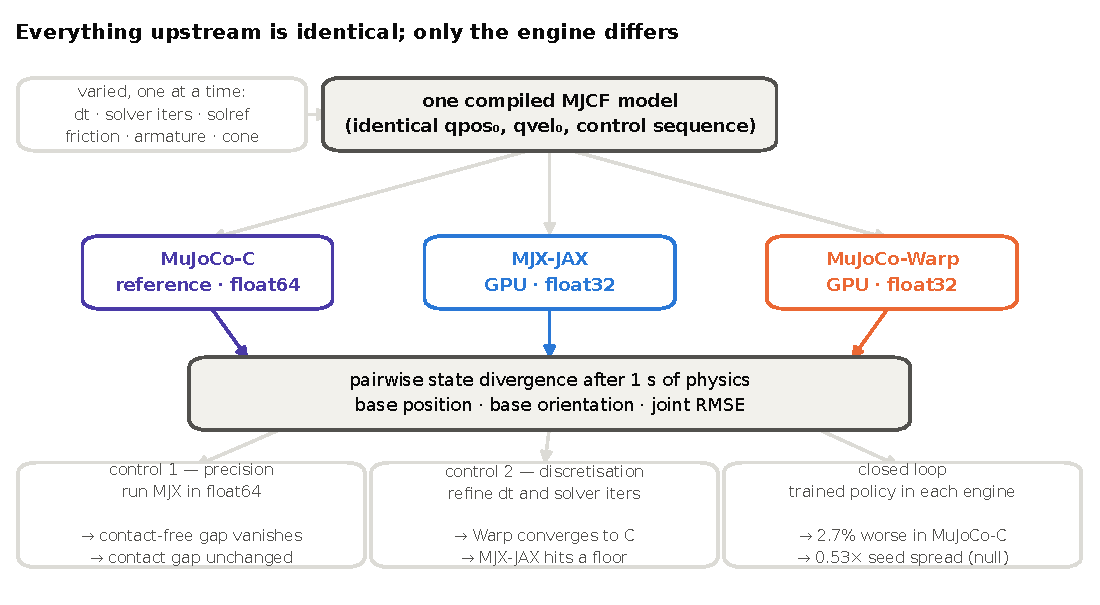
\includegraphics[width=\columnwidth]{fig6_schematic.pdf}
\caption{What is held fixed, what is varied, and what is measured. All
three engines are built from one compiled model and driven from the same
initial state and the same control sequence, so any difference in the
result belongs to the implementation.}
\label{fig:schematic}
\end{figure}

The three backends are MuJoCo~3.11.0 (C, float64), MJX~3.11.0 running on
JAX (GPU, float32), and MuJoCo Warp (CUDA, float32 only). Robots and
tasks come from MuJoCo Playground~0.2.0. Policies are PPO from Brax.

Figure~\ref{fig:schematic} shows the measurement. One MJCF model is
compiled once. All three engines are built from that same model and
stepped from identical joint positions and velocities under an identical
control sequence. We then measure how far the resulting states have
drifted apart after one second of physics, using base position error,
base orientation error, and joint RMSE. Because everything upstream is
shared, any difference is attributable to the engine.

\begin{table}[t]
\caption{The four bipeds, read from the models MuJoCo compiles rather than
from datasheets. Two columns anticipate later results: G1 is the only robot
declaring foot contact through explicit \texttt{<pair>} elements, and Op3 is
the only one shipping a coarse solver configuration.}
\label{tab:robots}
\centering
\tabfont
\begin{tabular}{@{}lccccc@{}}
\toprule
\textbf{Robot} & \textbf{Actuated} & \textbf{Mass} & \textbf{Height} &
\textbf{Contact} & \textbf{Shipped} \\
 & \textbf{DoF} & \textbf{(kg)} & \textbf{(m)} & \textbf{pairs} & \textbf{$dt$ / iters} \\
\midrule
Unitree G1        & 29 & 33.34 & 0.785 & \textbf{5} & 0.002 / 3 \\
Booster T1        & 23 & 31.61 & 0.665 & 0 & 0.002 / 3 \\
ROBOTIS Op3       & 20 & \phantom{0}3.15 & 0.244 & 0 & \textbf{0.004 / 1} \\
Berkeley Humanoid & 12 & 16.06 & 0.515 & 0 & 0.002 / 3 \\
\bottomrule
\end{tabular}
\end{table}

Table~\ref{tab:robots} lists the four bipeds. They span more than a factor
of ten in mass and better than two in actuated degrees of freedom, so
``humanoid'' covers a wide range here. Height is the base $z$ of the
keyframe each task resets to, which is the pose these comparisons start
from.

Two columns matter later. G1 is the only robot declaring foot contact
through explicit \verb|<pair>| elements, which is the correlation we test
directly in Section~\ref{sec:contactrep}. Op3 is the only one shipping
$dt=0.004$ with a single solver iteration, against $dt=0.002$ and three
iterations everywhere else, which turns out to explain its apparent
immunity to the whole effect.

Two design choices materially change the numbers, and we state them
because getting either wrong produces a confident wrong answer.

\textbf{We hold physical duration constant, not step count.} At a fixed
number of steps, $dt=0.004$ simulates 2.0~s of physics while $dt=0.001$
simulates 0.5~s. Divergence grows with simulated time, so fixing the step
count makes large timesteps look dominant for a trivial reason. Under a
fixed step count we first measured timestep at $109\times$ baseline. Held
to equal duration, the same condition is $1.50\pm0.49$, a null.

\textbf{We detect perturbations that do nothing.} Playground bipeds
declare foot--floor contact as explicit \verb|<pair>| elements, which
override per-geom values. Scaling \verb|geom_friction| alone therefore
changes nothing about the contacts carrying the robot, and would be
reported as a null. Each condition now asserts that it actually moved the
reference trajectory. None of the fourteen conditions triggered the guard.

%-----------------------------------------------------------------------
\section{Do the Engines Agree with Physics?}
\label{sec:groundtruth}

Before comparing engines to each other, we compare them to problems with
exact answers. This separates integrator error from contact-solver error
and gives an external reference.

A discrete integrator is not supposed to reproduce a continuous solution
exactly. Semi-implicit Euler on constant acceleration accumulates a known
offset of $g\,dt^2 n/2$ after $n$ steps. We therefore score against the
\emph{discrete} prediction, which is what separates a correct
implementation from a buggy one.

\begin{table}[t]
\caption{Accuracy against closed-form solutions. Without contact the two
GPU backends are identical to each other and differ from C only by
float32 rounding. With contact they separate.}
\label{tab:groundtruth}
\centering
\tabfont
\begin{tabular}{@{}lccc@{}}
\toprule
\textbf{Case} & \textbf{MuJoCo-C} & \textbf{MJX-JAX} & \textbf{MuJoCo Warp} \\
\midrule
\multicolumn{4}{@{}l}{\textit{Free fall}, 500 steps, error vs.\ discrete Euler (m)} \\
& $4.44\!\times\!10^{-15}$ & $6.97\!\times\!10^{-6}$ & $6.97\!\times\!10^{-6}$ \\[2pt]
\multicolumn{4}{@{}l}{\textit{Pendulum}, relative energy drift} \\
& $8.884\!\times\!10^{-4}$ & $8.891\!\times\!10^{-4}$ & $8.891\!\times\!10^{-4}$ \\[2pt]
\multicolumn{4}{@{}l}{\textit{Incline, sliding}, error vs.\ analytic $x$ (m)} \\
& $2.03\!\times\!10^{-3}$ & $2.12\!\times\!10^{-3}$ & $2.03\!\times\!10^{-3}$ \\[2pt]
\multicolumn{4}{@{}l}{\textit{Incline, static}, creep in 1~s (m), should be zero} \\
& $1.148\!\times\!10^{-3}$ & $1.128\!\times\!10^{-3}$ & $1.148\!\times\!10^{-3}$ \\
\bottomrule
\end{tabular}
\end{table}

\begin{figure}[t]
\centering
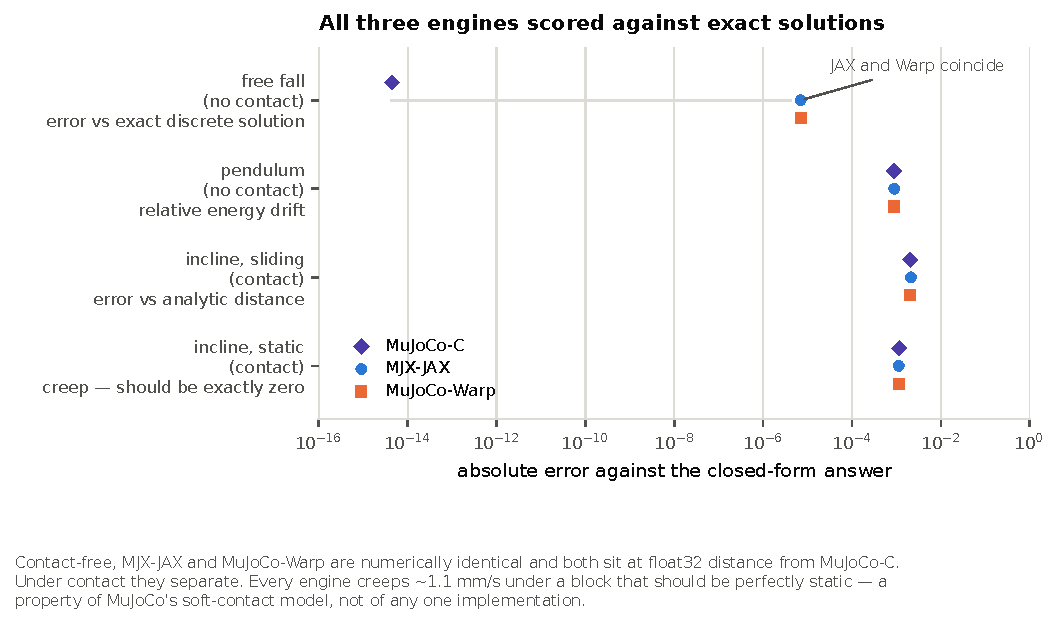
\includegraphics[width=\columnwidth]{fig5_groundtruth.pdf}
\caption{All three engines scored against closed-form solutions. MJX-JAX
and MuJoCo Warp land on top of each other in every case, which is itself
the finding; MuJoCo-C separates only where contact is absent, and there
the difference is float64 against float32.}
\label{fig:groundtruth}
\end{figure}

Table~\ref{tab:groundtruth} and Figure~\ref{fig:groundtruth} give the
result. In free fall, MuJoCo-C reproduces the discrete solution to
machine precision, while both GPU backends deviate by about
$7\times10^{-6}$---\emph{identically to each other}, which is the
signature of float32 against float64. All three share the same energy
drift to three significant figures, so that drift belongs to the
integrator, not to any engine.

Contact changes the picture. On the sliding block all three land within
0.18\% of the closed-form answer, yet Warp matches C to
$3.99\times10^{-6}$ while JAX sits $9.51\times10^{-5}$ away---a
$23.9\times$ difference in agreement among three engines that are all
``correct'' to within a fifth of a percent.

One result applies to everyone using this simulator. In the static case
the block must not move, and \emph{every} engine creeps about 1.1~mm in
one second. The magnitude is nearly identical across engines, so it comes
from MuJoCo's soft-contact model rather than from any implementation. For
locomotion that is a planted foot sliding roughly a centimetre over a
ten-second episode.

\textbf{What this establishes.} Without contact, the three engines agree
to float32 precision and the two GPU backends are indistinguishable. Any
larger disagreement on a humanoid is therefore about contact and
constraint solving, not arithmetic. This is the floor against which the
next section is read.

%-----------------------------------------------------------------------
\section{How Far Apart Are the Engines?}
\label{sec:howfar}

We now step a 29-DoF humanoid (\texttt{G1JoystickFlatTerrain};
$nq=36$, $nv=35$, $nu=29$) from an identical state under an identical
hold-pose control sequence, varying one physics option at a time.

\begin{table}[t]
\caption{Baseline disagreement on G1, over 10 initial conditions.
MJX-JAX is the outlier: Warp and C sit together, and JAX sits apart from
both.}
\label{tab:baseline}
\centering
\tabfont
\begin{tabular}{@{}lcc@{}}
\toprule
\textbf{Engine pair} & \textbf{Base position (m)} & \textbf{Base orientation (rad)} \\
\midrule
C $|$ JAX   & $3.354\!\times\!10^{-3} \pm 7.6\!\times\!10^{-4}$ & $6.381\!\times\!10^{-3} \pm 1.2\!\times\!10^{-3}$ \\
C $|$ Warp  & $\mathbf{4.120\!\times\!10^{-4}} \pm 8.6\!\times\!10^{-5}$ & $1.914\!\times\!10^{-3} \pm 4.4\!\times\!10^{-4}$ \\
JAX $|$ Warp & $3.385\!\times\!10^{-3} \pm 8.1\!\times\!10^{-4}$ & $6.468\!\times\!10^{-3} \pm 1.3\!\times\!10^{-3}$ \\
\bottomrule
\end{tabular}
\end{table}

Table~\ref{tab:baseline} shows Warp is about $8\times$ closer to the C
reference than JAX. The informative row is the third: JAX$|$Warp
($3.385\times10^{-3}$) is statistically identical to C$|$JAX
($3.354\times10^{-3}$). Warp and C sit together and JAX sits apart from
both, so JAX is the odd one out rather than the two GPU backends simply
differing from CPU.

\textbf{Contact stiffness controls the size of the effect.} Sweeping the
contact solver reference gives one monotonic trend: the Warp advantage
over JAX is $2.1\times$ with stiff contacts (\texttt{solref}~$\times0.5$),
$8.1\times$ at the default, and $28.2\times$ with soft contacts
(\texttt{solref}~$\times2.0$). Softer contacts give the constraint solver
more freedom, and MJX-JAX's solver is the one that uses it. A flat
recommendation to ``use Warp'' is therefore unsafe: the advantage is
weakest with hard contacts, which is exactly what practitioners reach for
when chasing hardware realism.

\textbf{Solver iterations do nothing.} Ten, fifty, and one hundred
iterations give identical divergence to four significant figures
($3.739\times10^{-3}$), all indistinguishable from the shipped default of
three. This knob is not worth tuning.

\subsection{One robot at default settings is not enough}

\begin{figure}[t]
\centering
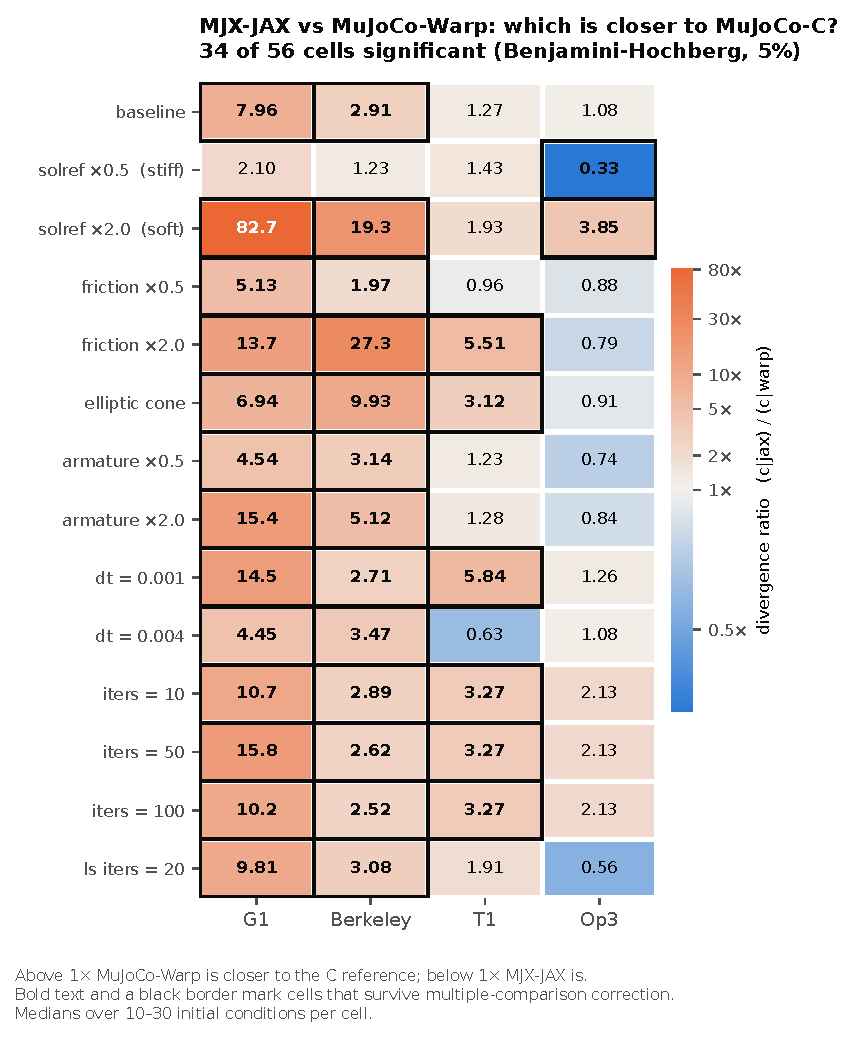
\includegraphics[width=0.86\columnwidth]{fig2_crossembodiment.pdf}
\caption{The full robot~$\times$~condition grid. 34 of 56 cells are
significant after Benjamini-Hochberg correction at 5\%. Reading only the
baseline row is what produced our own initial and wrong conclusion that
only G1 differs.}
\label{fig:crossembodiment}
\end{figure}

\begin{table}[t]
\caption{Cross-embodiment summary, medians with bootstrap intervals,
Benjamini-Hochberg over all 56 tests.}
\label{tab:crossembodiment}
\centering
\tabfont
\begin{tabular}{@{}lcc@{}}
\toprule
\textbf{Robot} & \textbf{Significant conditions} & \textbf{Median ratio} \\
\midrule
Unitree G1          & \textbf{13 / 14} & 10.23 \\
Berkeley Humanoid   & \textbf{13 / 14} & 3.08 \\
Booster T1          & 6 / 14 & 3.27 \\
ROBOTIS Op3         & 2 / 14 & 2.09 \\
\midrule
\textbf{Total}      & \textbf{34 / 56} & --- \\
\bottomrule
\end{tabular}
\end{table}

We repeated the sweep on every biped Playground ships.
Figure~\ref{fig:crossembodiment} and Table~\ref{tab:crossembodiment} give
the result: 34 of 56 cells are significant after correction, with
magnitudes from $2\times$ to $82\times$.

The important negative lesson is about protocol. Comparing engines at
each robot's shipped defaults---one cell of this grid, and exactly what a
single sim-to-sim check does---is not sufficient. T1 shows no advantage
at baseline (1.27, interval [0.64, 2.86]) but a significant one in six
other configurations. Reading robot-dependence off a single configuration
gave us the conclusion ``only G1 differs,'' which the full grid refutes.

Two qualifications matter. Op3 is largely null, so robot-to-robot
variation is real even if it is not the clean split a baseline-only
comparison suggests. And the effect is not universal in direction: Op3
under \texttt{solref\_scale=0.5} gives 0.33 [0.15, 0.89], significantly
\emph{below} one, meaning MJX-JAX is the closer backend there.

We considered and rejected the obvious alternative explanation, that T1
and Op3 simply diverge too little for a ratio to resolve. Their baseline
divergences are 13--45$\times$ smaller than G1's and Berkeley's, which is
suggestive. But T1's \emph{significant} conditions occur at its
\emph{smallest} divergences ($1.4$--$2.9\times10^{-4}$), while its two
largest-divergence conditions ($1.3$ and $1.9\times10^{-3}$) show nothing.
A measurement floor predicts the opposite ordering.

\subsection{Op3's immunity was its solver settings, not the robot}

Op3 ships with coarse defaults: $dt=0.004$ and one solver iteration,
against $dt=0.002$ and more iterations for the other three. We re-ran it
with settings matched to the rest, changing nothing else, and applied
Benjamini-Hochberg across the resulting 28 tests as one family.

\begin{table}[t]
\caption{ROBOTIS Op3 under its shipped settings and under settings
matched to the other three robots. Benjamini-Hochberg over the 28 tests
shown ($p \le 0.0232$).}
\label{tab:op3}
\centering
\tabfont
\begin{tabular}{@{}lcc@{}}
\toprule
\textbf{Setting} & \textbf{Significant} & \textbf{Median ratio} \\
\midrule
As shipped ($dt=0.004$, 1 iteration) & 1 / 14 & 3.85 \\
Matched ($dt=0.002$, more iterations) & \textbf{13 / 14} & 4.40 \\
\bottomrule
\end{tabular}
\end{table}

Table~\ref{tab:op3} shows the result: 1 of 14 becomes 13 of 14, with the
largest cell reaching $63.5\times$ [38.7, 114.8]. Op3's apparent immunity
was a property of its shipped configuration, not of the robot. Coarse
discretisation produces error large enough to hide the effect.

This has a direct practical reading. A sim-to-sim check run at a robot's
default settings can return a clean pass simply because those settings are
too coarse to resolve the disagreement.

%-----------------------------------------------------------------------
\section{Why the Engines Differ}
\label{sec:why}

The gap could be arithmetic (float32 against float64), discretisation
(finite step size and finite solver iterations), or algorithmic (the
implementations disagree about contact dynamics). We test the first two
directly. Each is ruled out while the gap stays.

\begin{figure*}[t]
\centering
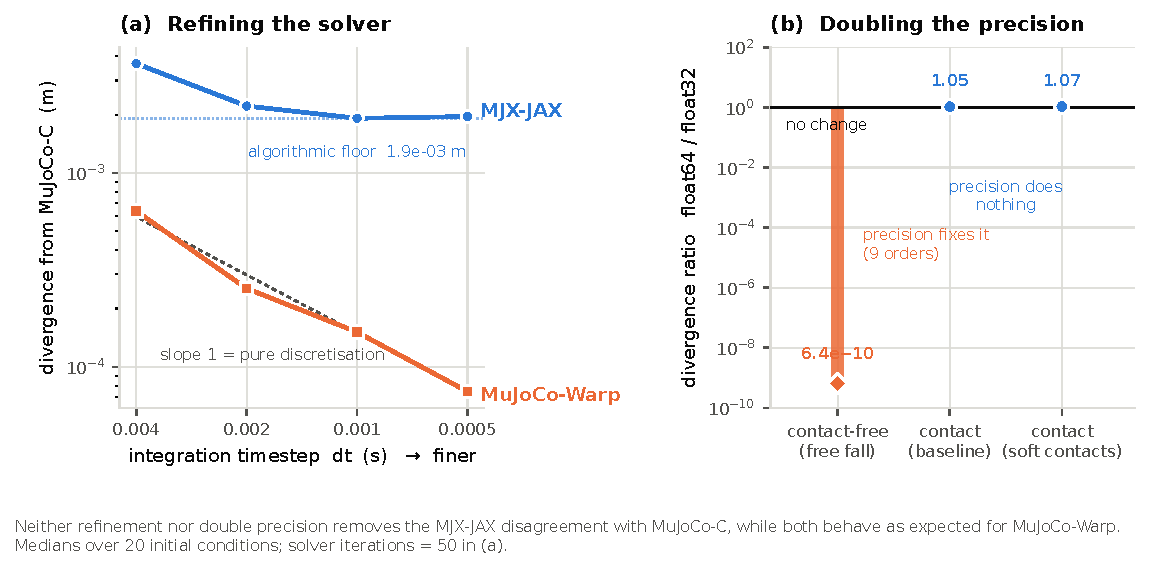
\includegraphics[width=0.92\textwidth]{fig1_algorithmic.pdf}
\caption{Two independent controls, one conclusion. (a) Refining the
timestep: MuJoCo Warp converges toward MuJoCo-C along slope~1, the
signature of a discretisation difference, while MJX-JAX flattens at a
floor. (b) Doubling the precision: float64 collapses the contact-free gap
by nine orders of magnitude, proving the manipulation works, and leaves
the contact gap untouched.}
\label{fig:algorithmic}
\end{figure*}

\subsection{It is not arithmetic}

We re-ran the C-versus-JAX comparison with JAX in double precision. Warp
rejects float64 arrays, so this is JAX-only, which is the relevant
comparison since JAX is the backend that departs from the reference.

The positive control is what makes this decisive. In float64 the
contact-free free-fall error falls from $6.97\times10^{-6}$ to
$4.441\times10^{-15}$, exactly matching MuJoCo-C. The precision change
demonstrably works. Without that control, ``float64 did not help'' would
be unfalsifiable.

\begin{table}[t]
\caption{Double precision does not close the contact gap. Medians over 20
initial conditions, base position error in metres.}
\label{tab:precision}
\centering
\tabfont
\begin{tabular}{@{}lccc@{}}
\toprule
\textbf{Condition} & \textbf{float32} & \textbf{float64} & \textbf{Ratio} \\
\midrule
baseline               & $1.921\!\times\!10^{-3}$ & $2.013\!\times\!10^{-3}$ & 1.048 \\
\texttt{solref}~$\times2.0$ & $3.101\!\times\!10^{-2}$ & $3.310\!\times\!10^{-2}$ & 1.067 \\
\texttt{solref}~$\times0.5$ & $2.928\!\times\!10^{-3}$ & $3.120\!\times\!10^{-3}$ & 1.065 \\
\texttt{friction}~$\times2.0$ & $2.236\!\times\!10^{-3}$ & $2.261\!\times\!10^{-3}$ & 1.011 \\
$dt=0.001$             & $1.955\!\times\!10^{-3}$ & $2.062\!\times\!10^{-3}$ & 1.055 \\
\midrule
\multicolumn{4}{@{}l}{\textit{Contact-free control} (free fall)} \\
free fall              & $6.97\!\times\!10^{-6}$ & $4.441\!\times\!10^{-15}$ & $6\!\times\!10^{-10}$ \\
\bottomrule
\end{tabular}
\end{table}

Table~\ref{tab:precision} and Figure~\ref{fig:algorithmic}(b) give the
answer. Every contact ratio is about 1.0, and if anything slightly above
it. The same switch that erases the contact-free gap by nine orders of
magnitude leaves the contact gap untouched. The disagreement is about
contact dynamics, not rounding.

This also changes the outlook. A precision difference would shrink as
hardware and libraries improve. An algorithmic one persists until an
implementation changes.

\subsection{It is not discretisation}

A difference that is only an artefact of finite step size should vanish
under refinement. We swept a $4\times4$ grid over $dt$ and solver
iterations, 20 initial conditions per cell.

Iterations saturate at three. Across every timestep the gap drops sharply
from one to three iterations and then stops moving, independently
reproducing the earlier result on a different grid. Playground's shipped
default of three is already converged.

\begin{table}[t]
\caption{Refining the timestep at 50 solver iterations. Warp converges
toward C; JAX stops at a floor. Base position error in metres.}
\label{tab:convergence}
\centering
\tabfont
\begin{tabular}{@{}lccc@{}}
\toprule
\textbf{$dt$ (s)} & \textbf{C $|$ JAX} & \textbf{C $|$ Warp} & \textbf{Warp step ratio} \\
\midrule
0.004  & $3.668\!\times\!10^{-3}$ & $6.359\!\times\!10^{-4}$ & --- \\
0.002  & $2.216\!\times\!10^{-3}$ & $2.536\!\times\!10^{-4}$ & 0.40 \\
0.001  & $1.915\!\times\!10^{-3}$ & $1.511\!\times\!10^{-4}$ & 0.60 \\
0.0005 & $\mathbf{1.956\!\times\!10^{-3}}$ & $\mathbf{7.459\!\times\!10^{-5}}$ & 0.49 \\
\bottomrule
\end{tabular}
\end{table}

Table~\ref{tab:convergence} and Figure~\ref{fig:algorithmic}(a) show the
two backends refining differently. Each halving of $dt$ roughly halves
Warp's gap, which is clean first-order convergence toward zero; an
eight-fold refinement yields an $8.5\times$ reduction. MJX-JAX falls to
about $1.9\times10^{-3}$ and stops, and its finest timestep is marginally
\emph{worse} than the next-coarsest. At the finest settings the MJX-JAX
gap is $26\times$ the Warp gap, and that ratio grows as refinement
continues.

\textbf{Two orthogonal controls, one conclusion.} Precision and
discretisation are independent knobs. Warp behaves as a discretisation
difference should under both. MJX-JAX behaves that way under neither. The
two implementations converge to different answers, which is what
``algorithmic'' means.

This also explains the cross-embodiment pattern. The Warp advantage is
visible wherever MJX-JAX's algorithmic floor dominates, and hidden
wherever discretisation error is large enough to mask it---which is
precisely why Op3's coarse shipped settings concealed it until they were
matched.

%-----------------------------------------------------------------------
\section{Does a Policy Notice?}
\label{sec:policy}

The physics differ. The question a robot-learning venue cares about is
whether a learned policy behaves differently. We ran two versions of the
test.

\textbf{Decision rule, fixed in advance.} A cross-backend gap is only a
finding if it exceeds the noise from ordinary training. Training three
seeds in one backend and evaluating each in both yields the effect and
its null model from the same runs. The verdict is
$|\text{gap}| / \text{seed noise}$: at least 2 is an effect, 1--2 is weak,
below 1 is no policy-level effect. The analysis script refuses to return a
verdict with fewer than two seeds.

\begin{figure}[t]
\centering
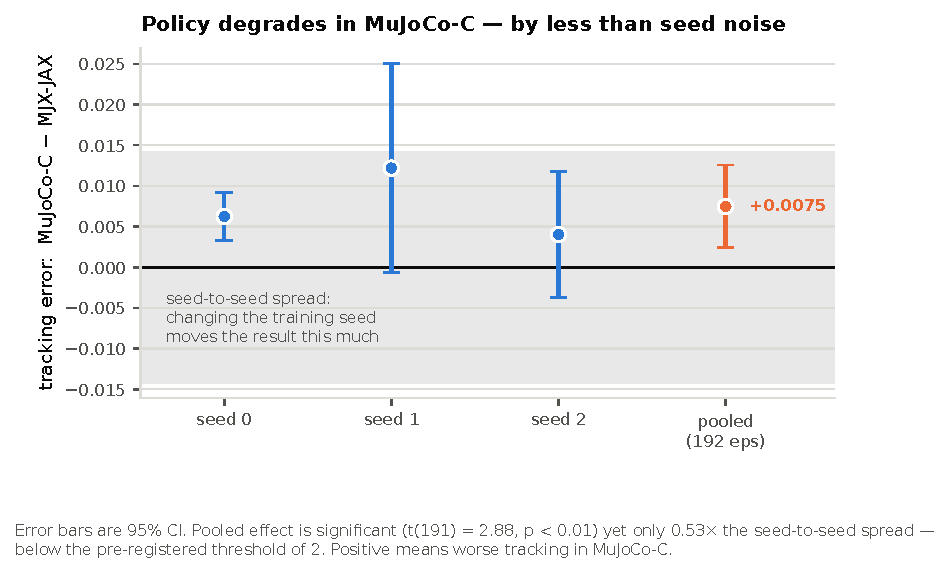
\includegraphics[width=\columnwidth]{fig3_policy_null.pdf}
\caption{The measured backend effect against the seed-to-seed variation it
has to be judged against. The effect falls inside the band that retraining
alone produces.}
\label{fig:policynull}
\end{figure}

\textbf{Test 1: JAX against Warp.} Three PPO policies (52.9M steps each,
512 environments) were evaluated in both backends over 128 episodes of
1000 steps, giving 384 matched pairs. The mean paired difference is
$+0.3264$ with $t(383)=1.400$, below the 1.96 threshold, and Cohen's
$d=+0.071$. The per-policy gaps do not even share a sign
($+0.431$, $-0.022$, $+0.570$). Against the pre-registered rule,
$|0.3264| / 0.5822 = 0.56$: no policy-level effect.
Figure~\ref{fig:policynull} shows why the comparison needs the null model:
the measured effect sits inside the band that retraining alone produces.

\textbf{Test 2: JAX against the C reference.} Test 1 compares two GPU
reimplementations of the same engine. The protocol in the literature
validates against MuJoCo-C, and Section~\ref{sec:howfar} shows that is
where the discrepancy lives, so the comparison that matters had not been
run. Playground environments are MJX-native, so we reproduced against
\verb|mujoco.MjData| the parts of the environment the policy depends on:
the 103-dimensional observation, the action-to-motor-target map, the gait
phase, and the termination condition.

\begin{table}[t]
\caption{Policy evaluated in MJX-JAX and in the MuJoCo-C reference, scored
on velocity-tracking error (lower is better). 64 paired episodes per seed.}
\label{tab:ceval}
\centering
\tabfont
\begin{tabular}{@{}lccccc@{}}
\toprule
\textbf{Seed} & \textbf{$n$} & \textbf{MJX-JAX} & \textbf{MuJoCo-C} & \textbf{Paired diff} & \textbf{$t$} \\
\midrule
0 & 64 & 0.2861 & 0.2923 & $+0.0062$ & 4.09 \\
1 & 64 & 0.2650 & 0.2771 & $+0.0122$ & 1.86 \\
2 & 64 & 0.2917 & 0.2958 & $+0.0040$ & 1.02 \\
\midrule
pooled & 192 & & & $\mathbf{+0.0075}$ & $\mathbf{2.877}$ \\
\bottomrule
\end{tabular}
\end{table}

That reimplementation matters enough to state its accuracy: it agrees
with MJX to $2.38\times10^{-7}$ on the full observation at reset and
$5.96\times10^{-8}$ on bookkeeping across 200 steps, with the gait phase
exact. Four bugs were found only because these checks existed, each of
which produced plausible output and no error---a frozen gait clock, an
off-by-one in the stored action and phase, an inverted termination test,
and a flaw in the validator itself.

Table~\ref{tab:ceval} gives the result, and two statements are
simultaneously true. There \emph{is} a systematic effect: pooled over 192
paired episodes the policy tracks worse in MuJoCo-C, $t(191)=2.877$,
consistent in sign across all three seeds, Cohen's $d=0.21$. And it
\emph{does not matter}: the difference of means (0.0075) is $0.53\times$
the seed-to-seed spread (0.0141), below the threshold of 2. We report the
null, as pre-registered, despite the paired test being significant.

\textbf{Trajectories diverge far more than returns do.} A single policy
rolled out from an identical state separates steadily: 0.019~m at 1~s,
0.068~m at 4~s, 0.190~m at 8~s, and 0.271~m at 10~s, against
$3.4\times10^{-3}$~m for open-loop control over 1~s. Closed-loop execution
amplifies the physics gap by roughly two orders of magnitude in state
space, and still leaves task performance unchanged. The policy is not
insensitive to the physics. It is robust in aggregate while being
individually unpredictable.

That distinction has a practical cost. Any claim resting on a specific
rollout---a demonstration video, a failure-case analysis, a worst-case
bound---is backend-dependent even though the aggregate is not.

%-----------------------------------------------------------------------
\section{How Much Divergence Can a Policy Absorb?}
\label{sec:dose}

The previous section answers yes or no for one engine pair. The question
underneath is quantitative: a policy trained in simulator A and run in B
loses performance as a function of how far apart they are. Where is the
knee, and is distance alone enough to describe it?

We characterise each perturbed configuration twice. The \emph{dose} is
the open-loop divergence between unperturbed and perturbed physics under
MuJoCo-C, the same quantity we measure between engines, so the two share
an axis. The \emph{response} is closed-loop task performance under the
perturbed physics. Three parameters were swept over 19 conditions, three
policy seeds, 64 episodes each.

Plotting against measured divergence rather than parameter value is what
makes this transferable. No other group's simulator pair is described by
our \texttt{solref\_scale}, but every pair can be located by how far apart
it is.

\begin{figure}[t]
\centering
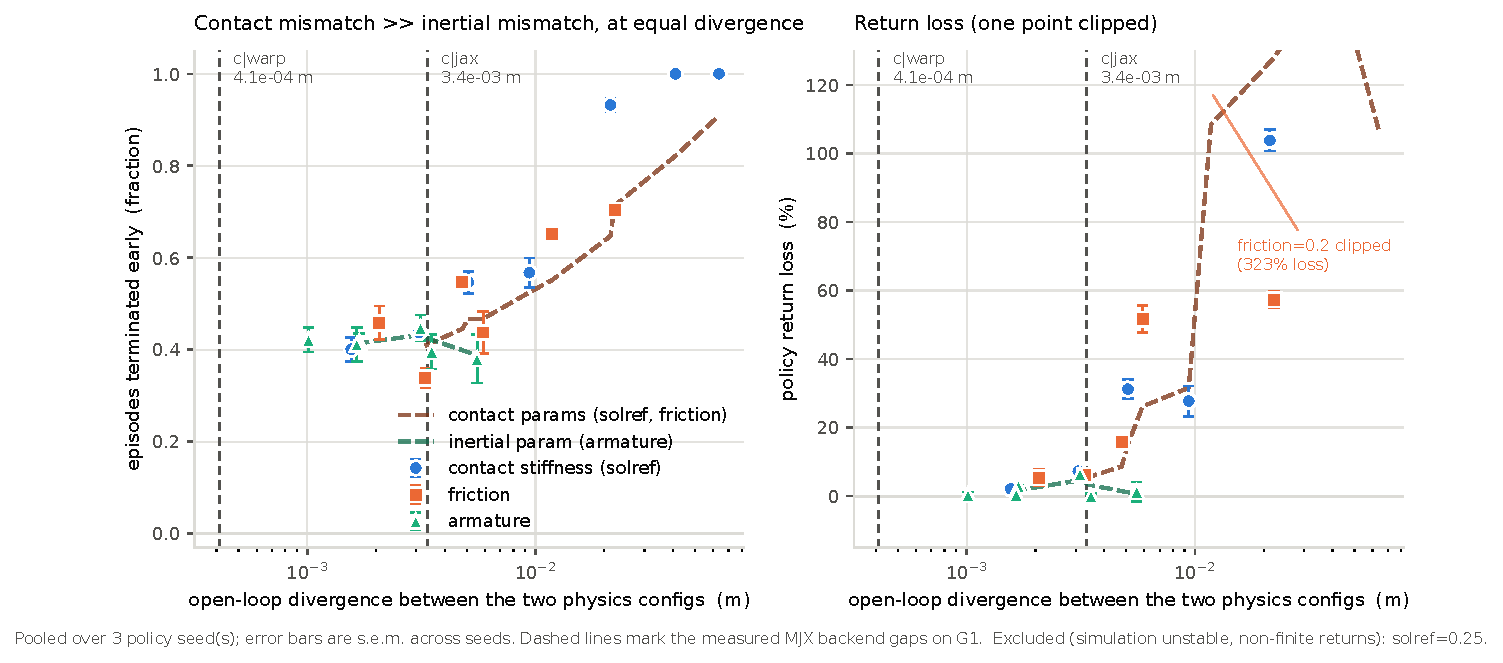
\includegraphics[width=\columnwidth]{fig4_tolerance.pdf}
\caption{Closed-loop cost against measured open-loop divergence, with the
real engine gaps marked on the same axis. Contact and inertial
perturbations of equal dose have very different consequences.}
\label{fig:tolerance}
\end{figure}

\begin{table}[t]
\caption{Within a parameter, divergence predicts loss. Across parameters,
it does not.}
\label{tab:dose}
\centering
\tabfont
\begin{tabular}{@{}lcc@{}}
\toprule
\textbf{Parameter} & \textbf{Spearman $\rho$} & \textbf{Loss range} \\
\midrule
\texttt{solref} (contact stiffness) & $\mathbf{+0.964}$ & 2.1--135.6\% \\
\texttt{friction} (contact)         & $\mathbf{+0.943}$ & 5.3--323.3\% \\
\texttt{armature} (joint inertia)   & $+0.143$ & $-0.0$--6.4\% \\
\bottomrule
\end{tabular}
\end{table}

Table~\ref{tab:dose} and Figure~\ref{fig:tolerance} give the result. At
matched dose the difference is stark: \texttt{friction=0.4}
(dose $5.90\times10^{-3}$~m) costs 51.7\%, while \texttt{armature=4.0}
(dose $5.55\times10^{-3}$~m) costs 1.3\%---a $40\times$ difference at the
same divergence. Armature never exceeds 6.4\% loss at any divergence we
tested.

\textbf{The headline is not a universal tolerance curve.} It is that
\emph{where} two simulators differ matters more than \emph{how much}. A
single scalar summary of simulator disagreement---which is what a naive
sim-to-sim check reports---cannot tell a benign inertial mismatch from a
damaging contact mismatch of identical size.

We expected the curves to collapse onto one, and drew that conclusion from
a partial sweep before the full condition set refuted it. The distinction
survives because it is mechanically sensible. Armature is a joint-space
inertia term that feedback compensates for. Contact parameters change how
the robot meets the ground, which feedback cannot recover from.

\textbf{This explains the null.} Section~\ref{sec:groundtruth} established
that the engine gap is specifically a contact-solver gap, so it belongs to
the damaging family. The contact curve predicts roughly 6--7\% loss at
G1's measured C$|$JAX gap of $3.35\times10^{-3}$~m. Against a noise floor
of 1.86\% and seed variation of comparable size, that is exactly the
regime in which the measurement returns a null. The null is not an absence
of physics. It is a predicted-size effect sitting at the resolution limit
of the measurement.

\textbf{One perturbation broke the simulator.} \texttt{solref\_scale=0.25}
(contacts four times stiffer) drove divergence to 1.01~m and returns to
NaN. We exclude it from the curve and report it separately, because ``the
simulator became unstable'' is a different statement from ``the policy
degraded.''

%-----------------------------------------------------------------------
\section{Is Contact Representation the Mechanism?}
\label{sec:contactrep}

G1 is the robot with the largest discrepancy and also the only one
declaring foot contact through explicit \verb|<pair>| elements rather than
geom--geom collision. That is a correlation across four robots with one
significant point, so we tested it directly instead of leaving it as
speculation.

We built two models of the same robot differing only in how the identical
contact is declared: as shipped, and with the floor--foot pairs deleted
and the foot geoms given collision flags carrying the pair's parameters.
Because geom--geom friction is combined between two geoms whereas a pair's
friction is used directly, we matched the floor's friction as well;
without that the converted model would silently have had different physics.

The control is what makes this clean: the two models are
\textbf{bit-identical under MuJoCo-C} (0.000 divergence across five
initial conditions), because C routes both declarations through the same
solver. Any difference the GPU backends show is therefore an
implementation artefact.

The Warp advantage survives the conversion: 5.96 [3.43, 13.13] as shipped
against 6.68 [4.54, 13.96] converted, intervals overlapping almost
entirely. Contact representation is not the mechanism. We eliminate the
hypothesis by construction rather than leaving it untested. The mechanism
behind G1's magnitude remains open; the remaining candidates (foot
geometry, robot scale, contact count) cannot be separated with four robots.

%-----------------------------------------------------------------------
\section{Measuring This Correctly Is Harder Than It Looks}
\label{sec:pitfalls}

\subsection{The evaluation noise floor}

Every comparison here rests on evaluations that are nominally
deterministic: fixed random keys, a deterministic policy, an unchanged
model. On GPU they are not reproducible. Repeating an identical
evaluation gives different returns, because floating-point reductions are
not associative and thread scheduling varies between launches.

\begin{table}[t]
\caption{Repeating an identical evaluation three times. The stack carries
an unstated uncertainty of this size.}
\label{tab:noisefloor}
\centering
\tabfont
\begin{tabular}{@{}lcc@{}}
\toprule
\textbf{Episodes} & \textbf{s.d. over 3 repeats} & \textbf{\% of mean} \\
\midrule
16  & 0.837 & 9.91\% \\
64  & 0.571 & 8.34\% \\
128 & 0.127 & \textbf{1.86\%} \\
\bottomrule
\end{tabular}
\end{table}

Table~\ref{tab:noisefloor} gives the measurement. At our evaluation
settings the floor is 1.86\% of the mean. We report it as a measurement
with three repeats and make no claim about how it scales, because three
samples estimate a standard deviation too poorly to support one. We note
it because it appears to be undocumented: a reported improvement smaller
than this is not distinguishable from a rerun.

\subsection{Four errors that produced confident wrong answers}

Each of the following ran without error, returned a plausible number, and
was wrong. We list them because none would have been caught by testing
that the code runs.

\begin{table}[t]
\caption{Protocol errors we made, what each produced, and the guard that
now makes it fail loudly.}
\label{tab:pitfalls}
\centering
\tabfont
\begin{tabular}{@{}p{0.28\columnwidth}p{0.28\columnwidth}p{0.30\columnwidth}@{}}
\toprule
\textbf{Error} & \textbf{Wrong answer} & \textbf{Guard} \\
\midrule
Fixed step count, not fixed duration &
$109\times$ timestep effect (truly $1.50\pm0.49$, null) &
Conditions specified by physical duration \\[3pt]
Mean over heavy-tailed divergence &
Berkeley ratio 3.32 (truly 2.91 [1.58, 4.51]) &
Medians with bootstrap intervals \\[3pt]
Null model with mismatched units &
$3.17\times$ effect on null data (truly 0.56) &
Systematic and per-episode tests separated \\[3pt]
Solver dropped constraints silently &
All Op3 sweeps physically wrong &
Rollout raises on constraint overflow \\
\bottomrule
\end{tabular}
\end{table}

Table~\ref{tab:pitfalls} summarises them. Two deserve a note.

The null-model error is the easiest to make. Our script divided the mean
absolute \emph{per-episode} difference by the seed-to-seed spread of
\emph{means}. Those have different units, and the ratio is inflated by
roughly the square root of the episode count. It reported a $3.17\times$
effect on data that contains none. The two questions need separately
matched nulls: a systematic shift is tested against between-seed variation
of means, and per-episode perturbation against within-backend episode
variation.

The constraint-overflow error is the most dangerous, because the failure
was silent by design. The MJX backends size their constraint buffer from
\texttt{njmax}. The default was too small for Op3's four box feet, so the
solver dropped constraints and returned physically wrong trajectories
while printing a warning to a file descriptor nothing was reading. Every
Op3 sweep before we caught it was invalid. The rollout wrapper now raises
rather than returning such a trajectory, and the corrupted outputs are
kept rather than deleted.

%-----------------------------------------------------------------------
\section{Limitations}

\textbf{No hardware.} We can rank engines by agreement with the C
reference and by accuracy on closed-form problems. We cannot say which is
closest to reality. This is the central limitation and it bounds every
claim above.

\textbf{One task.} The cross-embodiment results cover four robots, but all
policy-level results are flat-terrain joystick locomotion on G1. Section
\ref{sec:dose} shows the gap grows sharply with contact softness, so a
task with softer or more intermittent contact could cross the threshold
where performance does move.

\textbf{Statistical power.} $n=10$ resolves the $13\times$
contact-stiffness effect comfortably but not effects of size around
$1.5\times$. ``Null'' here means ``not resolved at this sample size,'' not
``absent.''

\textbf{Compute.} A 4~GB laptop GPU caps parallel environments at 512
(measured faster than 1024) and the training budget at 50M timesteps,
about one quarter of Playground's default for this task. Policies are
therefore not trained to convergence.

\textbf{Mechanism.} We show the disagreement is algorithmic and rule out
contact representation as the cause, but we do not identify which part of
the constraint solver differs. That requires reading both implementations
against each other and is future work.

%-----------------------------------------------------------------------
\section{Conclusion}

We audited the sim-to-sim check that stands in for hardware when hardware
is unavailable. Three findings stand out.

The three MuJoCo backends are not interchangeable under contact. MJX-JAX
departs from the C reference more than MuJoCo Warp does, in 34 of 56
robot~$\times$~condition tests across four bipeds, by factors of 2 to 82.
The cause is algorithmic rather than numerical: neither double precision
nor solver refinement removes it, while both behave exactly as expected
for Warp. We also rule out contact representation as the mechanism by
construction (Section~\ref{sec:contactrep}).

A trained policy absorbs that gap. The measured degradation, 2.7\%, is
real and consistent in sign, yet smaller than the variation from
retraining with a different seed. That is not luck. Contact mismatch is
roughly 40 times more damaging than inertial mismatch at equal divergence,
and the engine gap lands where a policy still tolerates it.

Together these make sim-to-sim agreement a weak test. It exercises a gap
below the level at which policies respond, so passing it is not strong
evidence. We suggest reporting the physics configuration the check was run
under, comparing any gap against seed-to-seed noise from the same runs,
and treating a pass at default settings with the same caution as Op3's,
whose apparent immunity was its own solver settings all along.

%-----------------------------------------------------------------------
\section*{Acknowledgment}

We thank the maintainers of MuJoCo, MJX, MuJoCo Warp, and MuJoCo
Playground for releasing the software this study measures.

\bibliographystyle{IEEEtran}
\bibliography{refs}

\end{document}
